\renewcommand{\thesection}{Advanced Task}
\section{Deep Ice Skating using Deep Q-Learning}
\subsection{Environment}
The environment used for the Basic Task is too basic to implement Deep Q Learning. Instead, we created a more complicated ice rink environment, taking inspiration from the  same concept of the environment used in the Basic Task.

The agent is now located in a circular ice skating rink dojo which contains non-integer locations.
They are also using real ice skates that cannot easily control turning velocity.
Instead, each agent can accelerate or deaccelerate their turning speed at each turn.
In addition to the turning restrictions, the agent must constantly go forward at a constant speed and cannot stop or slow down at any point.

For reference, \textbf{\cref{circle_plots}} shows the result of one of our models in the environment.

When skating, the state consists of 4 floating point values and the state has 3 different actions.

\begin{center}
	\begin{minipage}[t]{.48\textwidth}
		\begin{center}
			\textbf{States}
		\end{center}
		\begin{description}[noitemsep,style=nextline]
			\item[\bm{$y$}] The $y$ coordinate of the agent.
			\item[\bm{$x$}] The $x$ coordinate of the agent.
			\item[\bm{$\varphi$}] The current angular the agent is at.
			\item[\bm{$\theta$}] The current angular velocity.
		\end{description}
	\end{minipage}
	\begin{minipage}[t]{.48\textwidth}
		\begin{center}
			\textbf{Actions}
		\end{center}
		\begin{description}[noitemsep]
			\item[0. Turn Left] Decrease angular velocity.
			\item[1. Stay Put] Keep angular velocity.
			\item[2. Turn Right] Increase angular velocity.
		\end{description}
	\end{minipage}
\end{center}

An agent starts at a random point of the ice dojo facing at a random direction but not turning.
Its objective is to get to the centre as fast as possible.
This dojo is finite: if the agent goes far enough, it will fall off the flat earth and the game is terminated.

The state and transitions functions are defined in the following equation.
\newcommand{\statet}{\left< y, x, \varphi, \theta \right>}
\begin{gather*}
	\state = \statet \\
	\begin{aligned}
		y'(\state, a) &= y + \frac{1}{4} \sin(\varphi'(\state, a)) \\
		x'(\state, a) &= x + \frac{1}{4} \cos(\varphi'(\state, a)) \\
		\varphi'(\state, a) &= \varphi + \theta'(\state, a)
	\end{aligned}
	\qquad
	\theta'(\state, a)= \begin{cases}
		\theta^t - \frac{1}{10} \pi & \text{if } a = 0 \\
		\theta^t & \text{if } a = 1 \\
		\theta^t + \frac{1}{10} \pi & \text{if } a = 2
	\end{cases} \\[1ex]
	T(\state, a) = \left< y'(\state, a), x'(\state, a), \varphi'(\state, a), \theta'(\state, a) \right>
\end{gather*}

The reward function is defined to maximise the changes of an agent making it to the centre by, in addition to giving high scores for winning and low scores for losing, giving it a score depending on the distance to the centre.
\begin{equation*}
	\reward(\state) = \begin{cases}
		\phantom{+}1000 & \text{if } \sqrt{y^2 + x^2} \leq \text{min distance} \\
		-1000 & \text{if } \sqrt{y^2 + x^2} \geq \text{max distance} \\[1ex]
		-\sqrt{y^2 + x^2} & \text{otherwise}
	\end{cases}
\end{equation*}

Adding a reward that depends on the distance considerably improved training speed and precision of the Deep Q-network compared to just subtracting a constant each time. Even though the results ``should'' be the same, subtracting the distance disincentives the agent from attempting bad solutions.

\newpage{}
\subsection{Implementation}
We implement a 3-layer Deep Q-network with hidden size set as a hyperparameter that's trained using an epsilon-greedy policy whose $\varepsilon$ value goes down linearly from a certain $\varepsilon$-start to 0.
The data used to train the model is accumulated and later randomly sampled from a large replay buffer. The original network (target = DQN) produces good solutions if trained in large batch sizes for a large amount of episodes.

% Frustratingly, it takes a very long time to even make ``passable'' solutions. In order to improve these convergence time, we present two improvements that can be alternatively added to this model.

Furthermore, we have deviated slightly in training the agent from the conventional method learnt in labs. Rather than training just 1 agent, we have opted to instead train multiple agents at the same time per episode, denoted by the variable "batch\_size", which is set to 5000. This ensures that our results gained from the training are consistent and not just a one-off case.

\subsection{Improvements}
% For the improvements we have implemented two algorithms, mainly the target network method and the Double-DQN method. Both of the methods vary slightly in the implementation algorithm, but may have impacting results if implemented right.

\subsubsection{Target Network}
The target network method introduces a new variable called the target network. The target network is initialised as an exact copy of the main network otherwise used in the conventional DQN method, but instead of updating every timestep, the target network is instead updated every certain timesteps, denoted by the variable update frequency, hence causing the target network to always lag behind the main network in terms of training.
The target network in this method evaluates the action made by the main network, calculating the best action and its Q-values using the formula:
\begin{align*}
    Q_{\text{target}}(s, a ; \theta^{-}) = r + \gamma \max_{a'} Q(s', a' ; \theta^{-})
\end{align*}

Evaluating the actions of the main network using the target network aims to increase the stability of the overall training of the agent.

\subsubsection{Double DQN}
The double-DQN method (DDQN) similarly utilises the target network used by the target method method, but it differs in the sense that instead of getting the best actions and its q-values like the aforementioned two methods, the DDQN method gets the best action through the main network, but calculates the q-values using the target network, using the following formula:
\begin{align*}
    Q^{\text{DDQN}}(s, a ; \theta) = \mathbb{E}_{s' \sim \varepsilon}[r + \gamma Q(s', \underset{a'}{\text{argmax}}\ Q(s', a ; \theta_{\text{target}}) ; \theta)]
\end{align*}
By doing so, the DDQN method aims to mitigate overestimation bias problems from the traditional DQN method, where the agent tends to overestimate the Q-values obtained during training. By doing so, DDQN methods generally tend to converge faster than the DQN method due to the agent not being stuck at repeating suboptimal actions that do not yield the best results but appeared in the first few episodes.

\subsection{Experiment}
To observe how the different parameters affect the performance of the agents, we have conducted a parameter search between the methods, hidden size, learning rate, discount factor $\gamma$ and initial epsilon decay. Every other parameters, such as the the batch size, action size and update frequency are kept the same to ensure consistency. 

\subsection{Analysis of Results}

\Cref{best_results_t2} presents the best 2 results for each method, which can be used to choose candidates.
\definecolor{id1}{rgb}{0.651,0.808,0.890}
\definecolor{id2}{rgb}{0.122,0.471,0.706}
\definecolor{id3}{rgb}{0.698,0.875,0.541}
\definecolor{id4}{rgb}{0.200,0.627,0.173}
\definecolor{id5}{rgb}{0.984,0.604,0.600}
\definecolor{id6}{rgb}{0.890,0.102,0.110}
\begin{table}[h]
	\centering
	\scriptsize
	\begin{tabular}{c c c c c c | c c c c}
		\toprule
		ID & method & hidden size & lr & gamma & $\varepsilon$-start & win rate & best episode & loss & q step \\
  \midrule
		\colorbox{id1}{1} & DQN & 256 & 0.001 & 0.99 & 0.5 & 1 & 178 & 10030k & 7091.87 \\
		\colorbox{id2}{2} & DQN & 512 & 0.001 & 0.99 & 0.8 & 1 & 197 & \phantom{0}8306k & 4608.34 \\
		\colorbox{id3}{3} & Target Network & 512 & 0.001 & 0.99 & 0.8 & 1 & \phantom{0}94 & 17494k & 6114.58 \\
		\colorbox{id4}{4} & Target Network & 512 & 0.001 & 0.99 & 0.5 & 1 & 124 & 12819k & 6709.36 \\
		\colorbox{id5}{5} & Double DQN & 512 & 0.001 & 0.99 & 1 & 1 & 101 & 22431k & 4119.00 \\
		\colorbox{id6}{6} & Double DQN & 512 & 0.001 & 0.99 & 0.8 & 1 & 107 & 13977k & 7215.91 \\
  \bottomrule
  \end{tabular}
	\caption{Candidate networks which will be plotted in \cref{candidate_comparison}, color coded for consistency with the plots.}
	\label{best_results_t2}
\end{table}

\subsubsection{Observations}
Observing \cref{best_results_t2}, both of the Target Network and DDQN method outperforms the DQN method in terms of convergence speeds. This is because both methods were able to mitigate the overestimation of the Q-values compared to the DQN method through the target network.

\subsubsection{Hidden sizes}
Generally, the hidden size of 512 is preferred over 256. This proves that a higher hidden size allows agents to have more dimensionality in computing the best actions in the environment, leading the agent to be able to accomodate for a higher variety of actions. Care should be taken however, that too high of a hidden size will cause the model to overfit, which fortunately is not the case in this project.

\subsubsection{Gamma values}
For all cases, gamma = 0.99 is preferred over 0.9. The higher gamma value prioritises future rewards, while the lower gamma values value immediate rewards higher. For the advanced task, despite the complexity of the environment, the environment is still considered deterministic, where discount factors are not needed, as seen in \cite{DRL_Hands_On}. In which case, since the agent is able to accurately calculate the rewards in its actions, higher gamma values allow the agent to learn the environment more thoroughly. However, in stochastic environments, a lower gamma value may be preferred due to the unpredictability of the agent when picking an action.

\subsection{Quantitative Analysis}
\label{candidate_comparison}

\begin{figure}[h]
	\begin{subfigure}{\textwidth}
		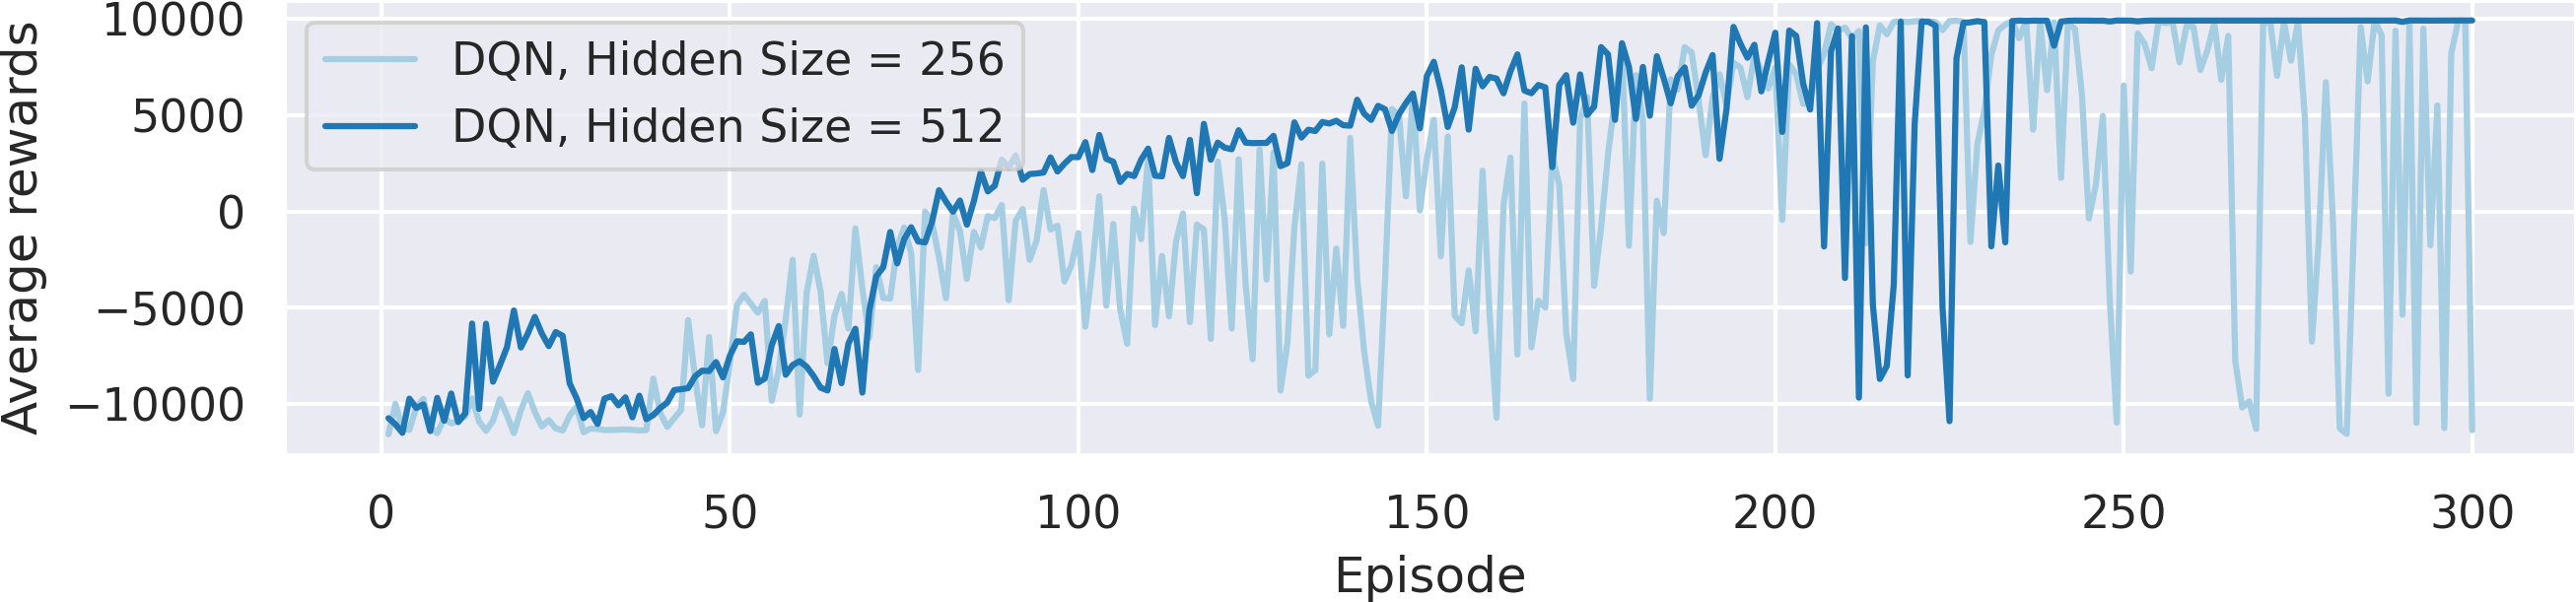
\includegraphics[width=\textwidth]{dqn_reward_size.png}
		\caption{Models using DQN.}
		\label{dqn_avg_reward}
	\end{subfigure} \\[1ex]
	\begin{subfigure}{\textwidth}
		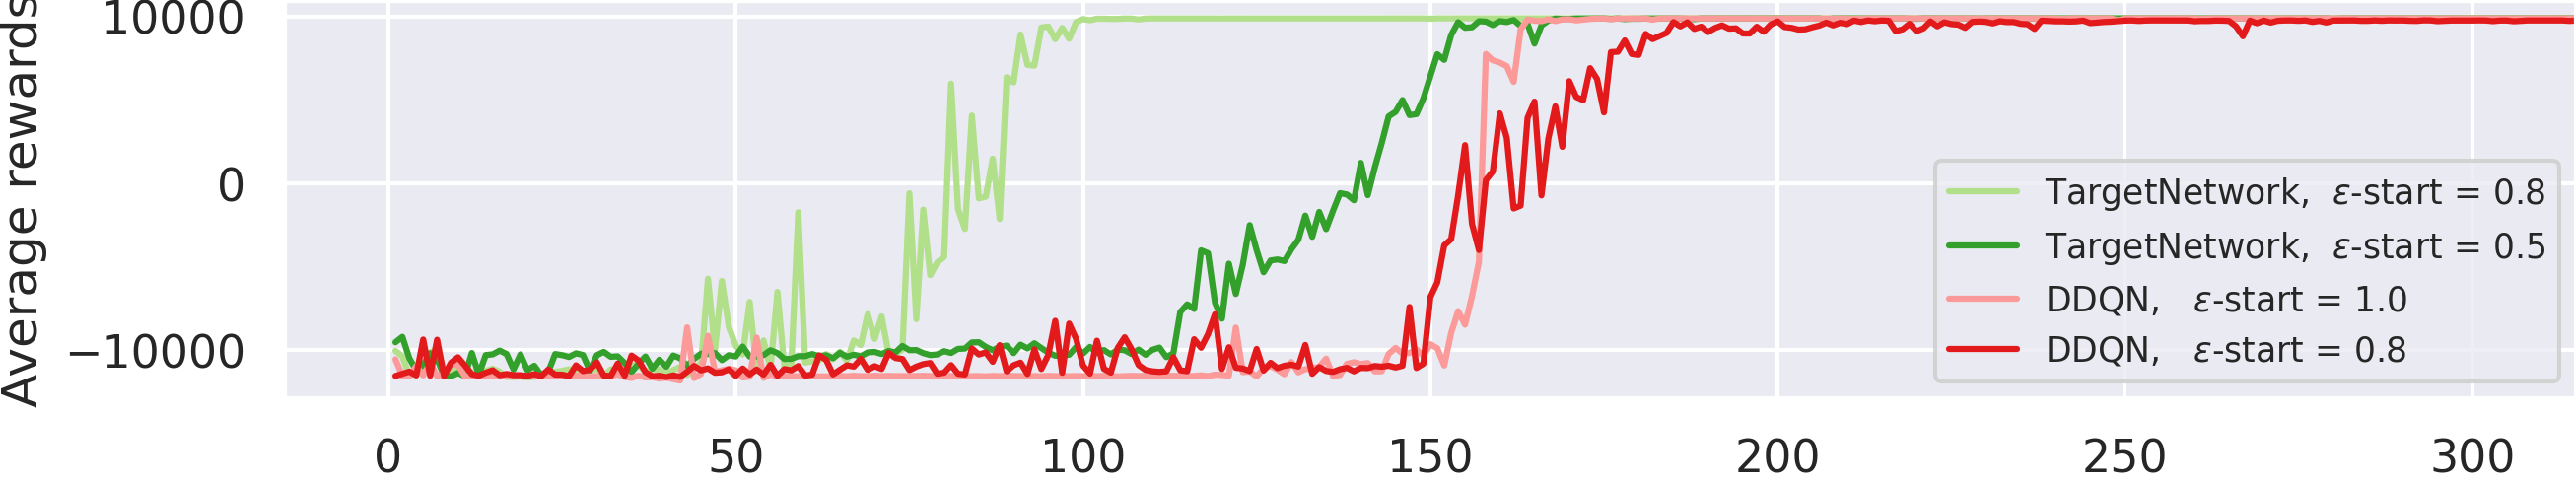
\includegraphics[width=\textwidth]{rest_reward_size.png}
		\caption{Models using DDQN and Target Network.}
		\label{rest_avg_reward}
	\end{subfigure}
	\caption{Reward sizes for the models presented in \cref{best_results_t2}.}
	\label{avg_reward}
\end{figure}

We made further experiments to the results in \cref{best_results_t2} to find patterns by running several trials in validation sets of 500 episodes each.
The trials are averaged and the first 300 episodes are shown, since nothing interesting happens afterwards.
Note that the validation sets are agents independent of training; their results are never random regardless of the value of $\varepsilon$ at that episode.

\Cref{avg_reward} shows the average reward for each one of the models by epoch.
As expected, the DQN values in \cref{dqn_avg_reward} are extremely chaotic: while both models converge to having a high reward, the average at every episode seems random.
This is due to the innate instability of DQN\cite{reinforcement_learning_introduction}.

In contrast, \cref{rest_avg_reward} shows that the average rewards in both target network and DDQN models are much better behaved with all models reaching a perfect score quickly and not moving from there. This is expected due to reasons explained above.

For this environment Target Network seems to converge much faster than DDQN. This might be due to the conditions favoring the Target Network more, with the environment and the hyperparameters such as the learning rate, update frequency and replay buffer capacity working better for the Target Network than the DDQN.


% As seem in \cref{losses}, the loss of all models goes down in time except for the DDQN with $\varepsilon\text{-start} = 1.0$, whose loss shoots up and only comes down when the model converges.

% This is likely due to the high initial epsilon of that set of parameters, where the model is still exploring and struggles to adapt to the environment
% \begin{figure}[h]
% 	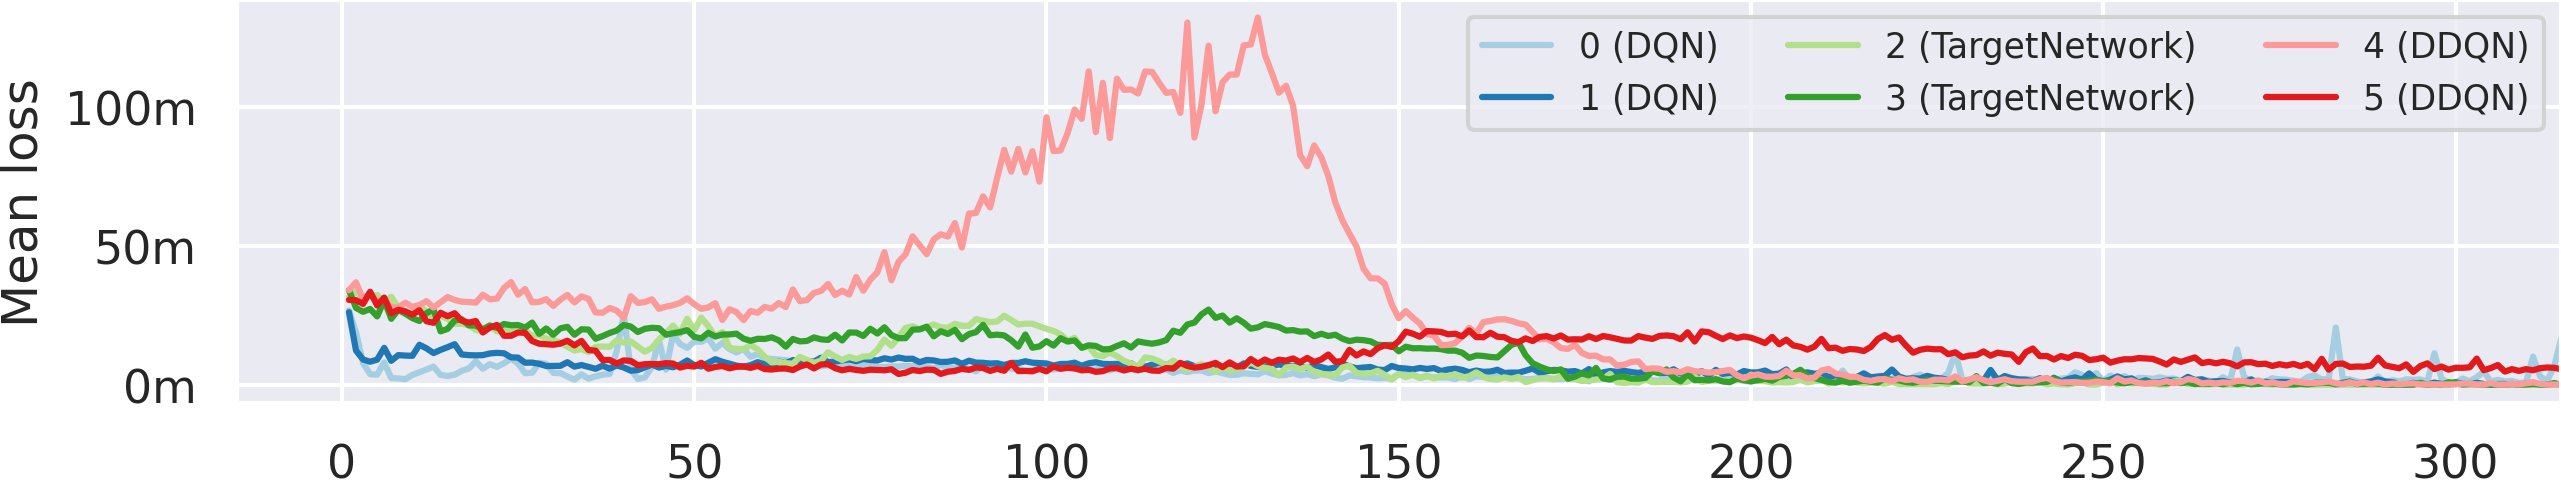
\includegraphics[width=\textwidth]{losses.png}
% 	\caption{Average loss of each model at each episode, with the mysterious loss spike for the DDQN with ID 4.}
% 	\label{losses}
% \end{figure}


\begin{figure}[h]
	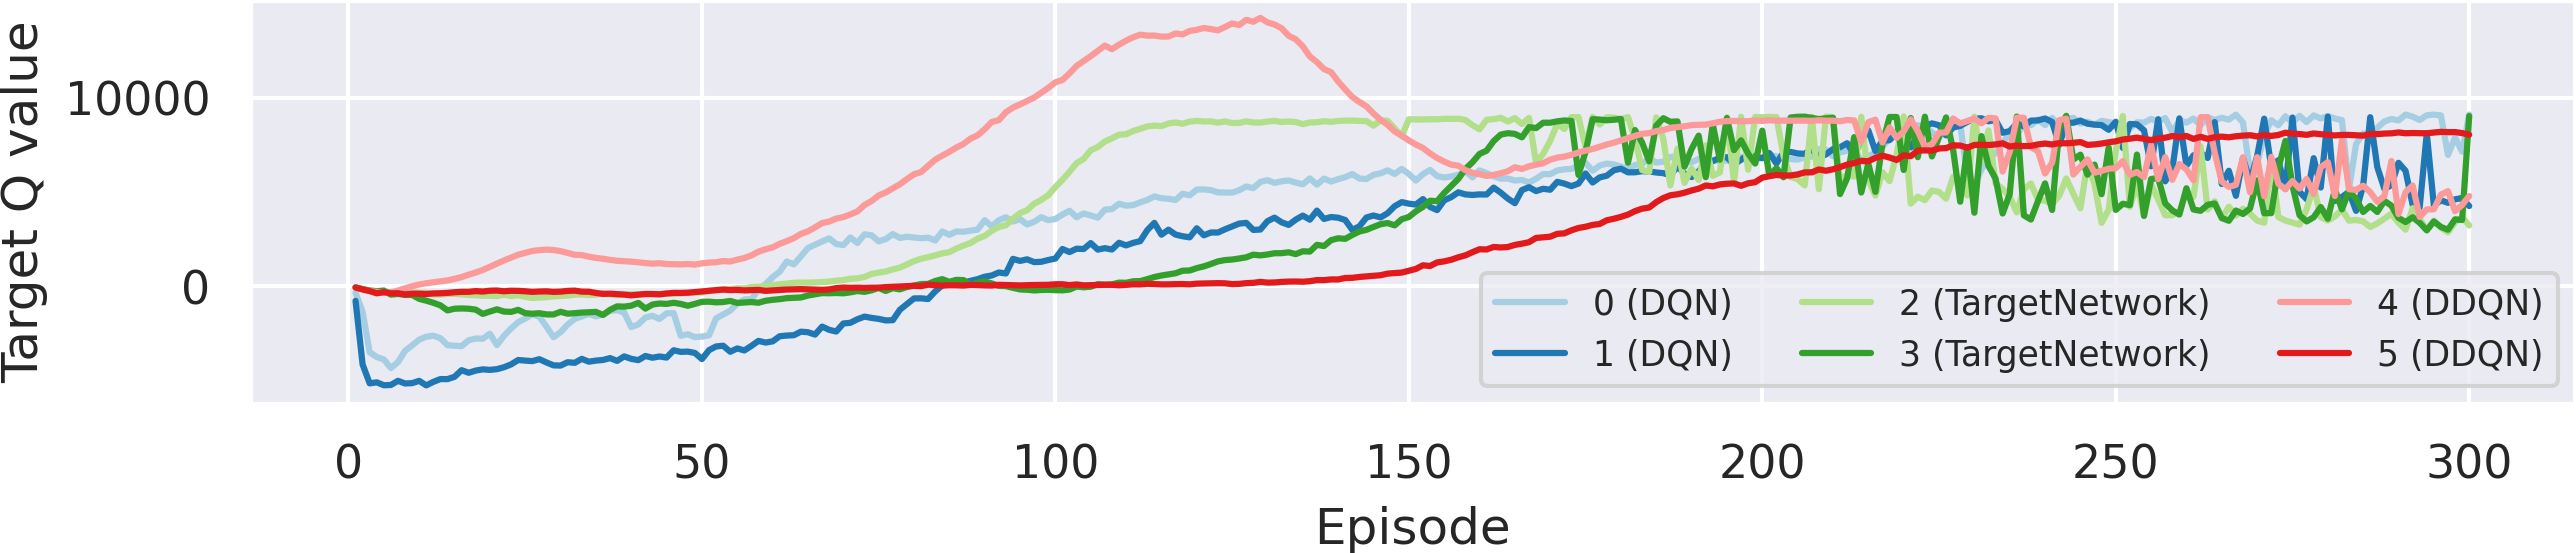
\includegraphics[width=\textwidth]{q_values.png}
	% \caption{Mean expected Q values of the models per episode.}
	\label{q_values}
\end{figure}

The expected Q values at each train, shown in \cref{q_values}, show a good example of the stability of the models: the ones for DDQN are smoother than the ones using TargetNetwork, which are in turn smoother than the ones using DQN, with exceptions to \colorbox{id5}{5}, which is likely due to the initial epsilon, where this particular DDQN is still exploring due to initial epsilon = 1 while the other 5 algorithms have already begun exploiting. The smooth Q values are expected from DDQN first and foremost, and this is true with the other DDQN set, where the agent sees a smooth transition to the maximum achievable Q-values compared to the other two methods.

In conclusion, we can infer from the results alone that the target network provides faster convergence, while the DDQN offers smoother convergence when calculating the q-values and losses, both of which are considered improvements over the regular DQN method.

\subsection{Qualitative Analysis}

However, what does it mean for a candidate to be better than another?

\Cref{circle_plots} shows 4 examples of the model with ID = 1 in \cref{best_results_t2} at different training episodes.
At each one of these episodes, 10 skaters are thrown in the environment with the objective of reaching the centre in as little time as possible.
These are validation skaters that use the model alone and are unaffected by $\varepsilon$.

\begin{figure}[H]
	\begin{subfigure}[t]{.32\textwidth}
		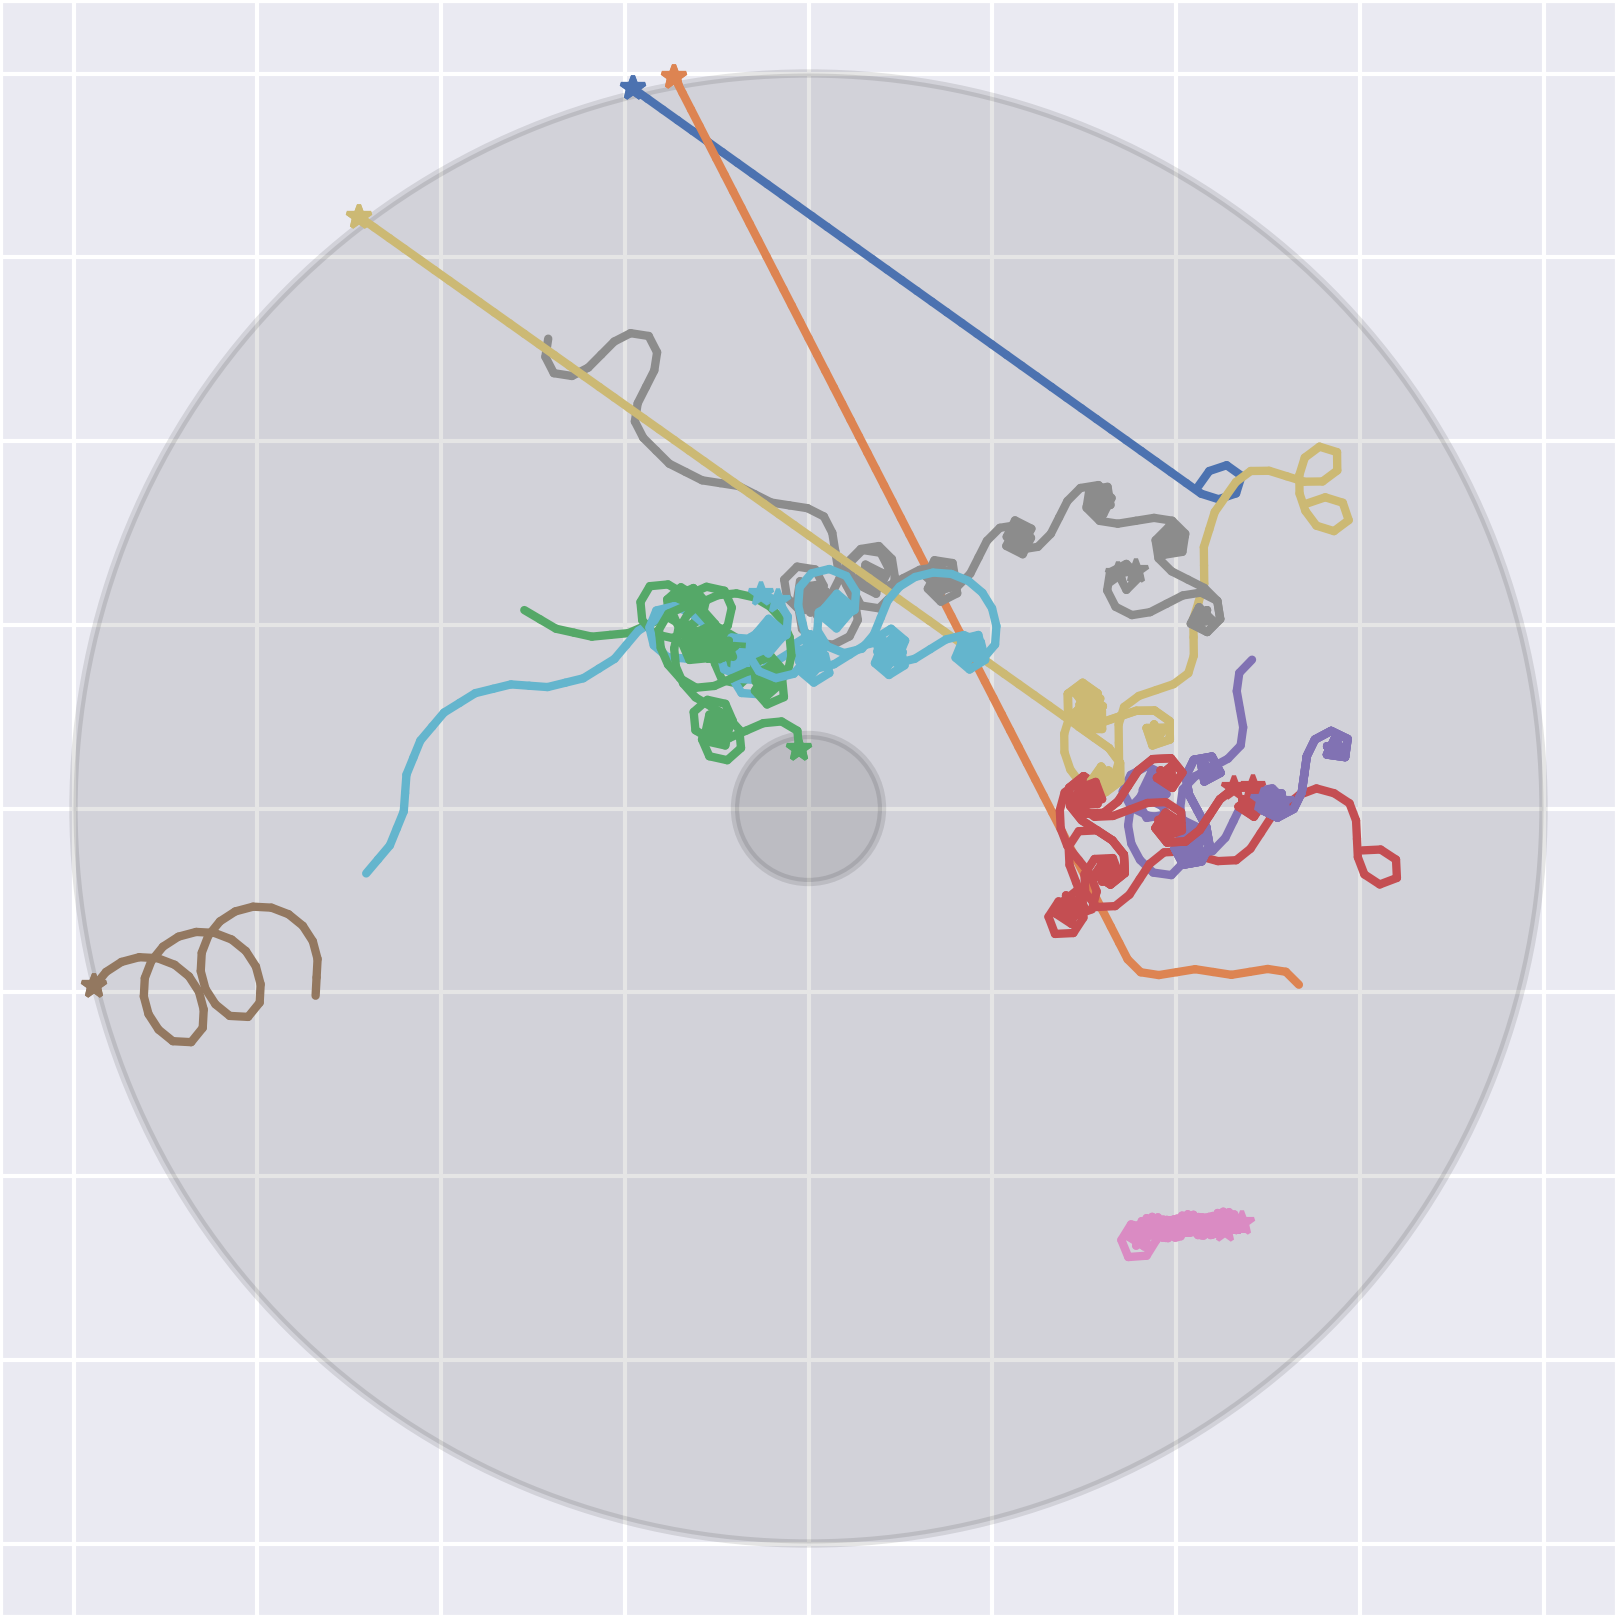
\includegraphics[width=\textwidth]{circle_images/image_50.png}
		\caption{State of the learners after \textbf{50 episodes}. The skaters act without much of a pattern, but there is one that reached the objective in the centre. Luck or intelligence?}
	\end{subfigure}\hfill{}
	% \begin{subfigure}[t]{.32\textwidth}
	% 	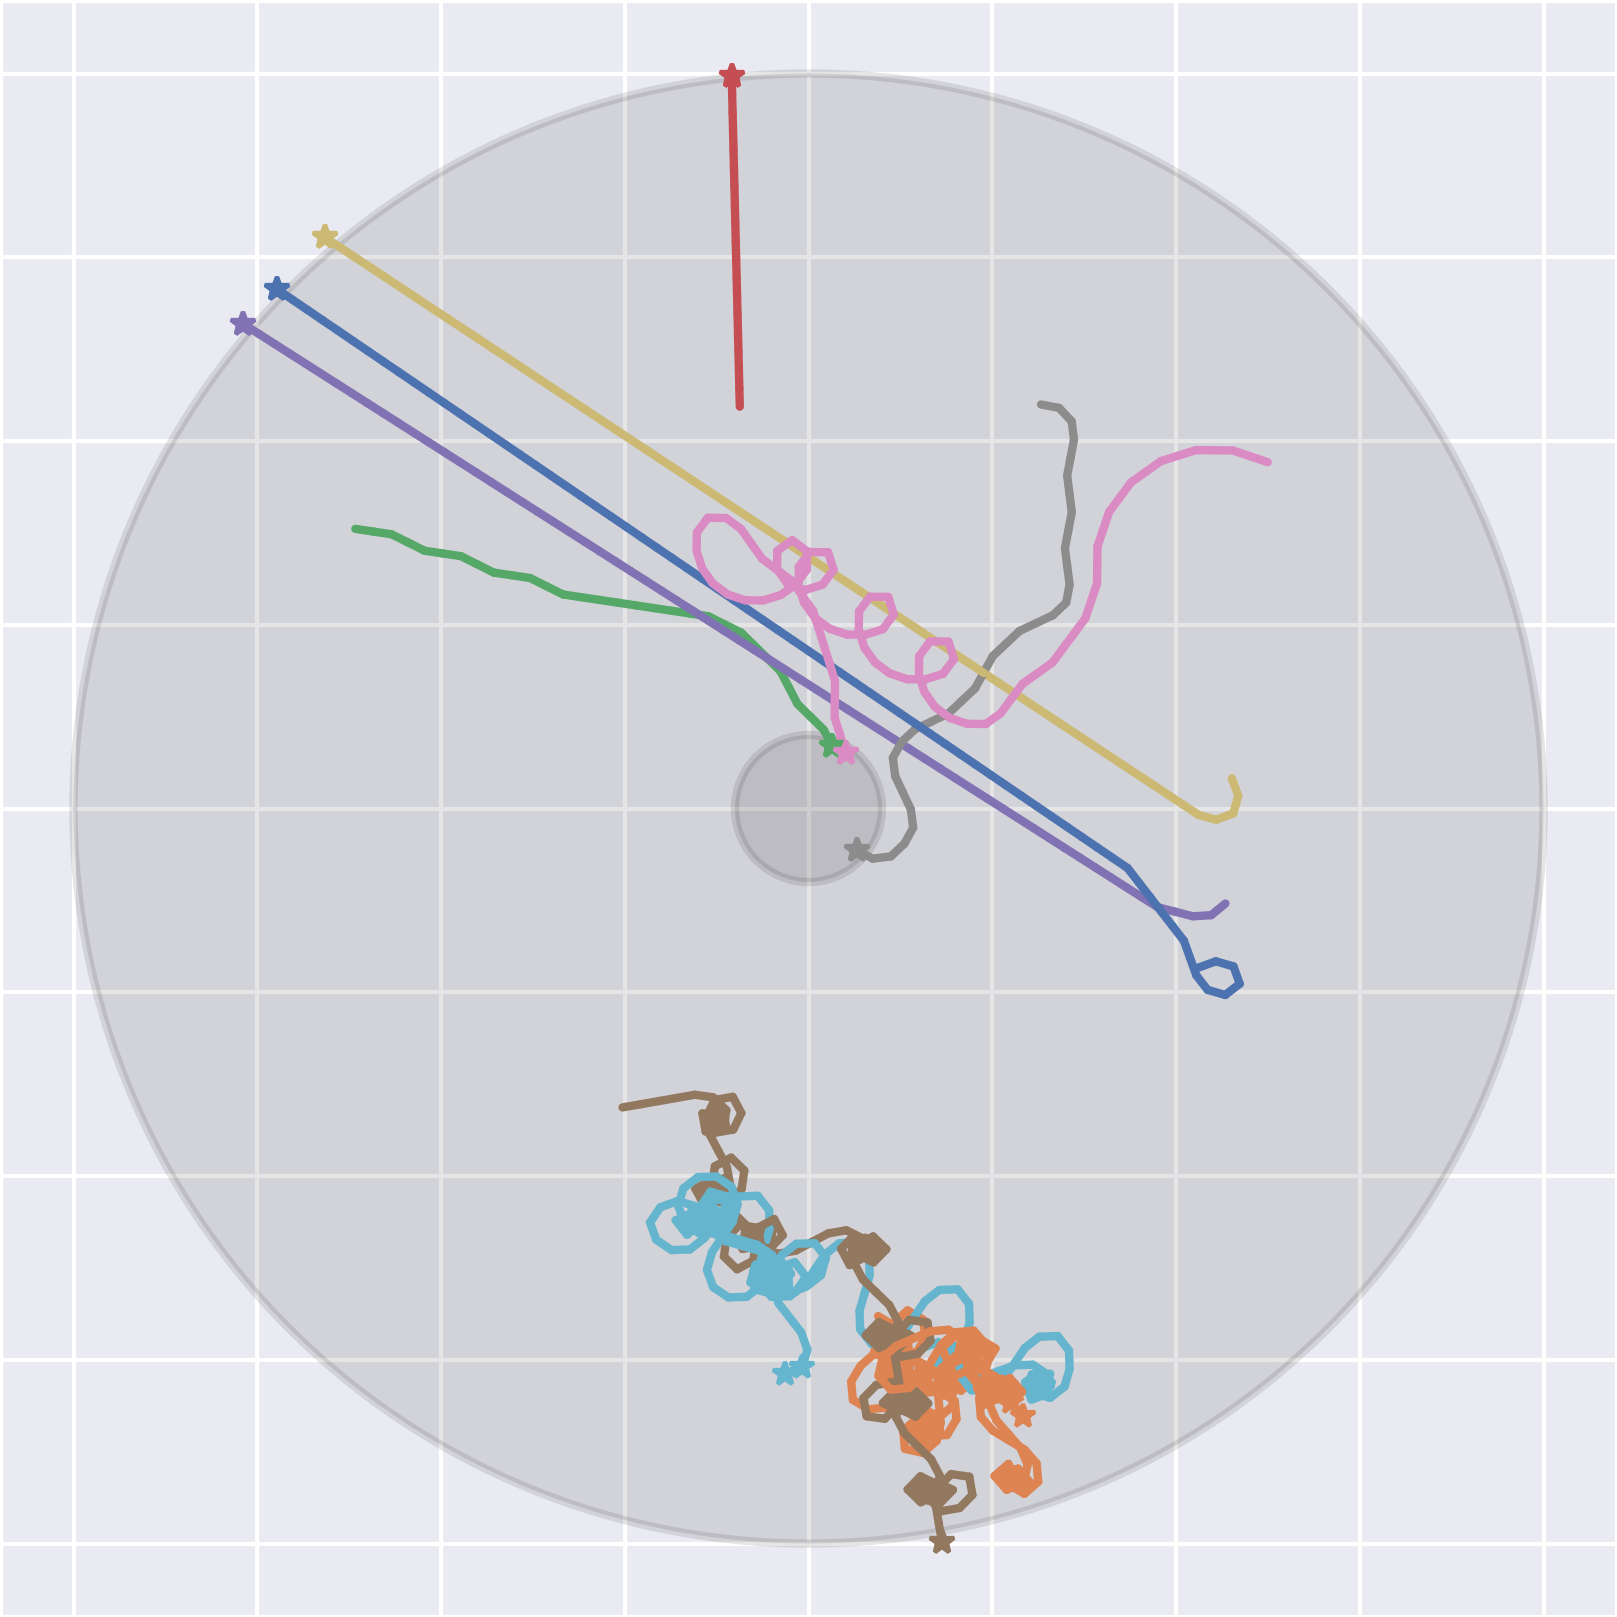
\includegraphics[width=\textwidth]{circle_images/image_100_alt_2.png}
	% 	\caption{State of the learners after \textbf{100 episodes}. Skaters travel in a not-necessarily-straight path to the centre if they are close, or basically random if they are far. Additionally, some agents pass close to the centre but do not turn towards it.}
	% \end{subfigure} \\
	\begin{subfigure}[t]{.32\textwidth}
		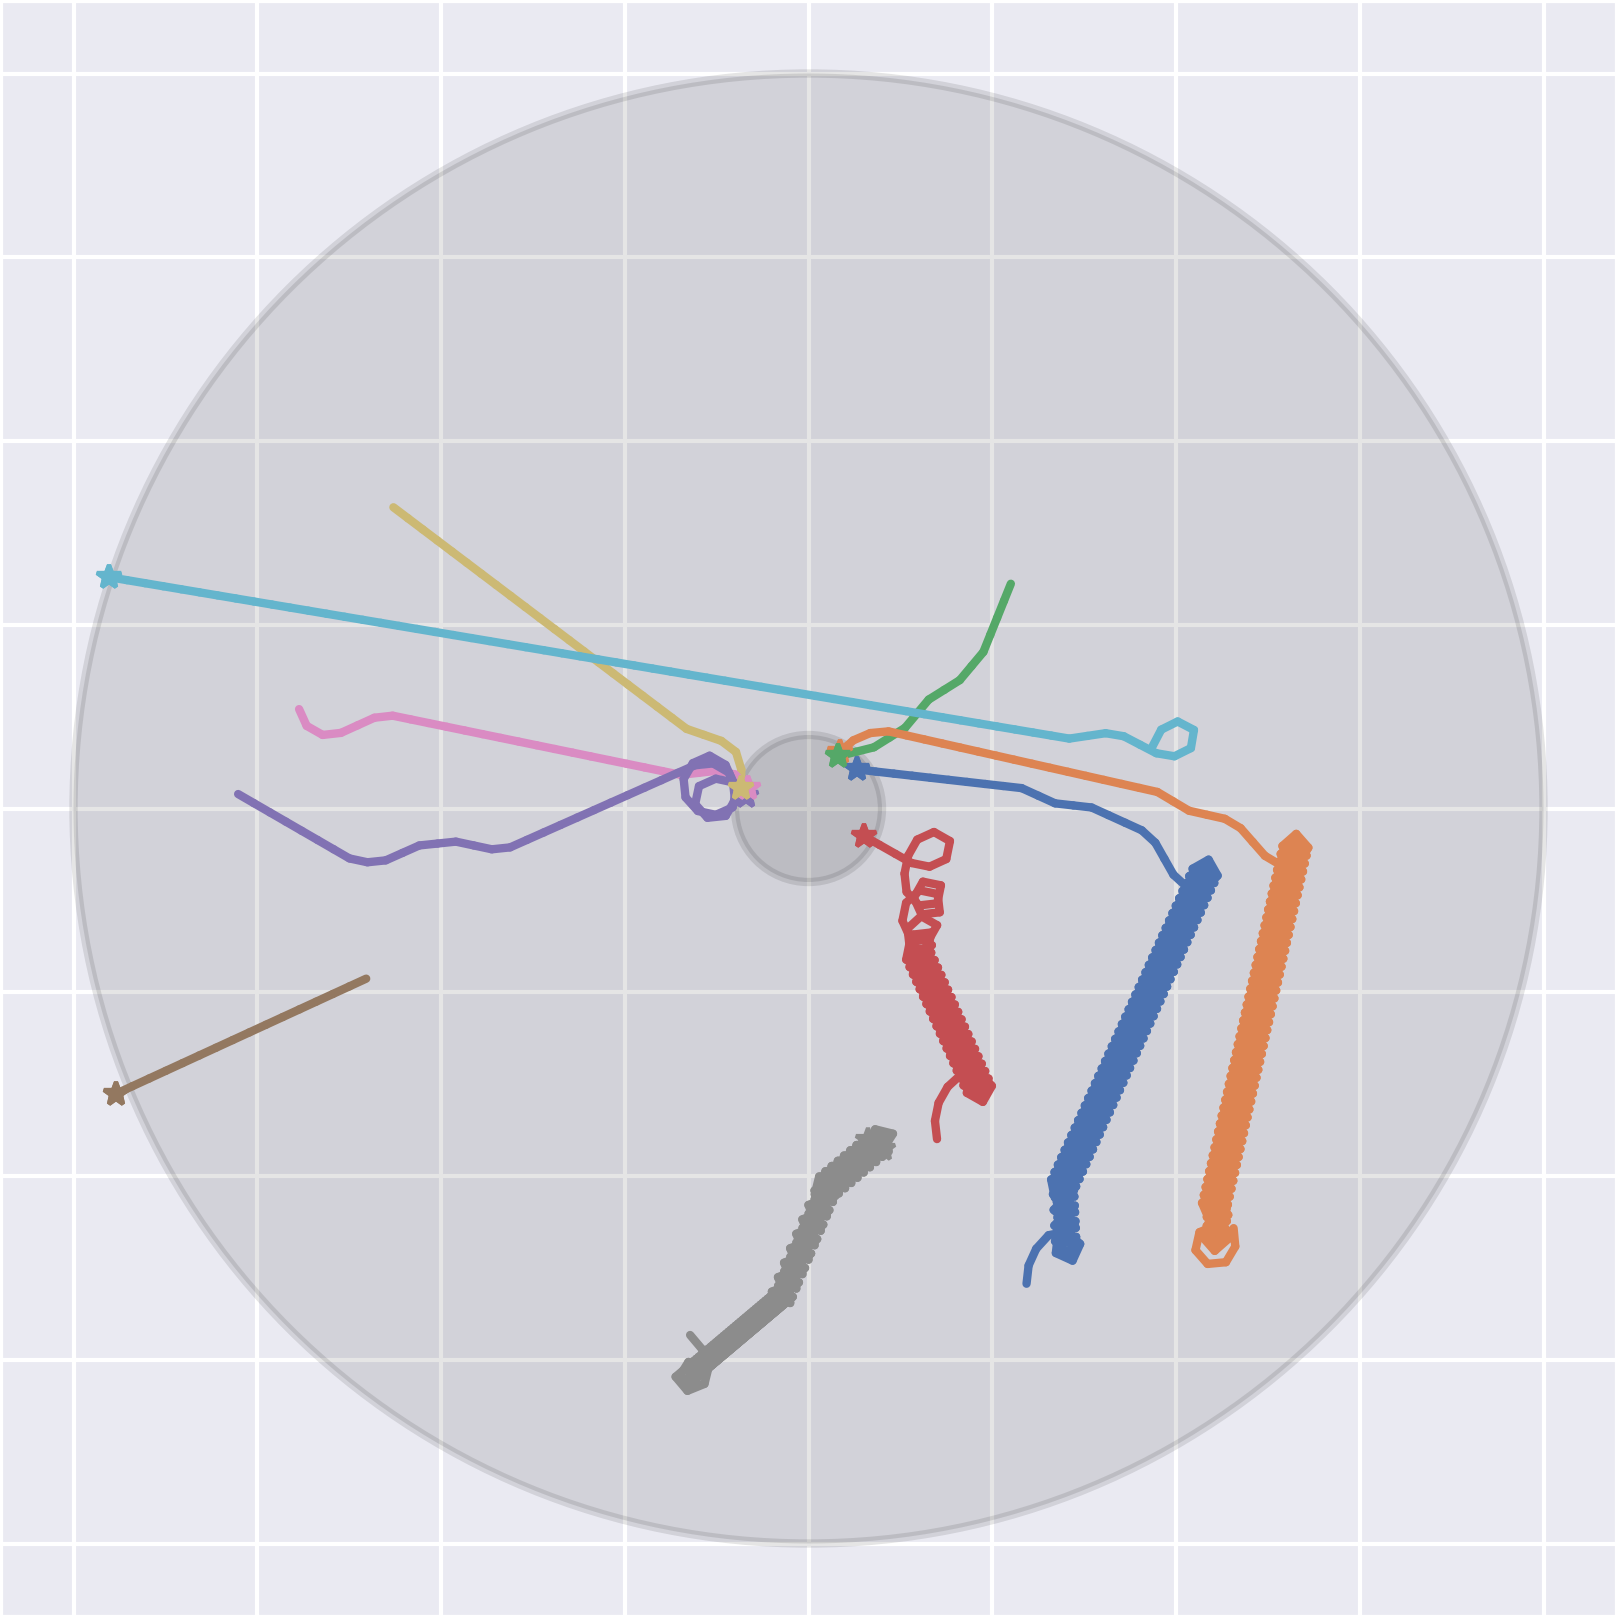
\includegraphics[width=\textwidth]{circle_images/image_150.png}
		\caption{State of the learners after \textbf{150 episodes}. Most skaters reach the centre, even if some of them get desperate their angular velocity at first, affecting their score.}
	\end{subfigure}\hfill{}
	\begin{subfigure}[t]{.32\textwidth}
		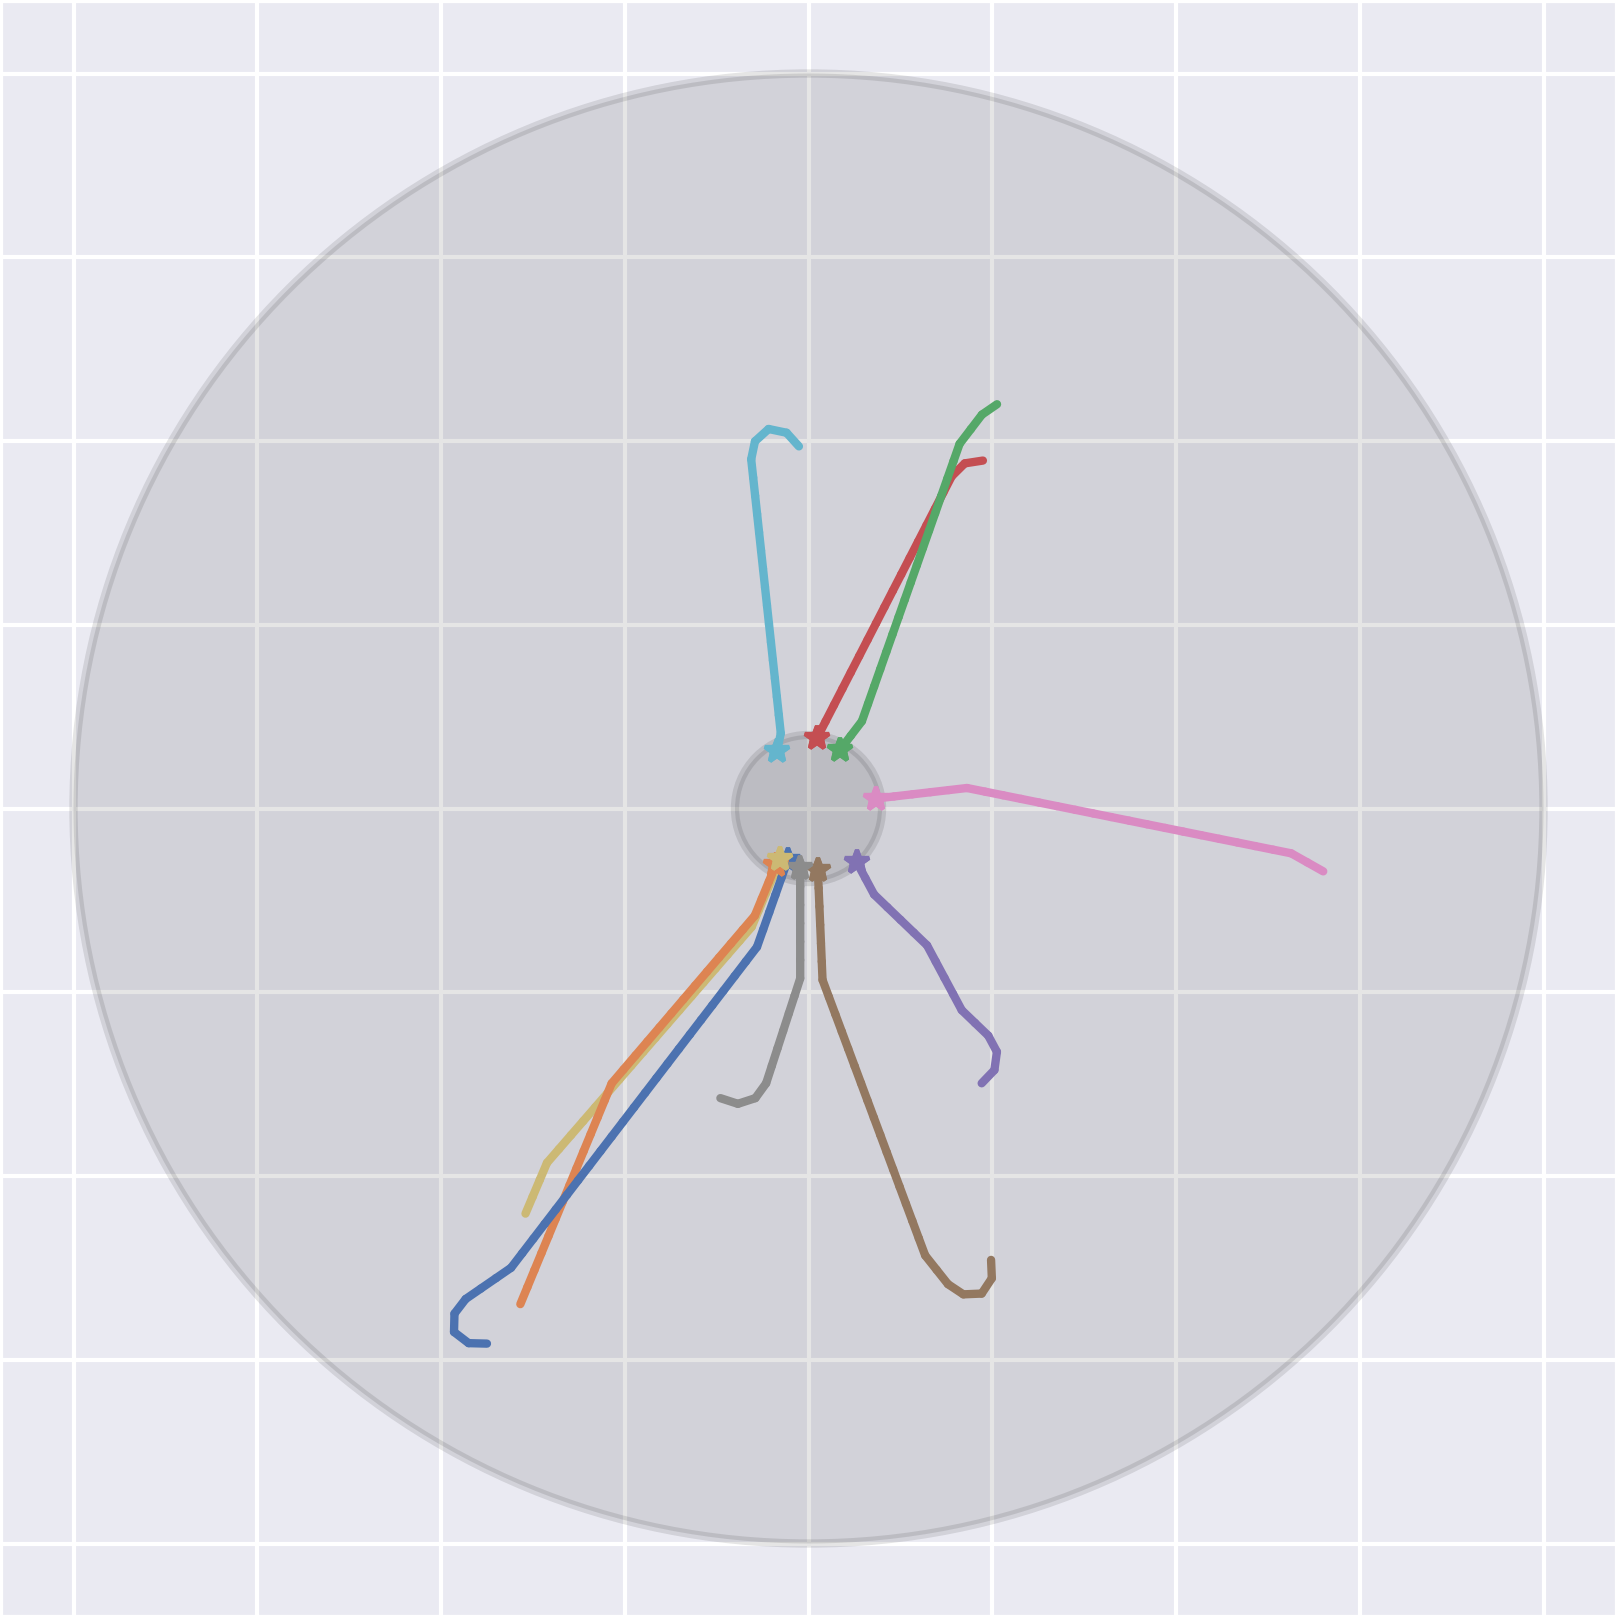
\includegraphics[width=\textwidth]{circle_images/image_300.png}
		\caption{After \textbf{300 episodes}, the skaters always find the shortest path to the centre regardless of where they start or in which direction they initially face.}
	\end{subfigure}
	\caption{Ice skating ice skating using DQN with hidden size = 512 (model \colorbox{id1}{1} in \cref{best_results_t2}).}
	\label{circle_plots}
\end{figure}
